\section{Design}
	\subsection{System Architecture Overview}
		The system will comprise of three main components:
		\begin{itemize}
			\item Management Server
			\item User Interface
			\item Disposable instances/containers
		\end{itemize}
		The system will also use existing infrastructure. This is where the backups are stored. Depending on the user of the system there may be multiple backup server in different location (such as AWS regions) or for different data types (relational and non-relational databases). Backup data may be stored in a variety of ways such as on EC2 instance or S3 buckets.
		
		\begin{figure}[H]
			\setlength{\belowcaptionskip}{15pt plus 3pt minus 2pt}
			\caption{Diagram of System Architecture}
			\centering
			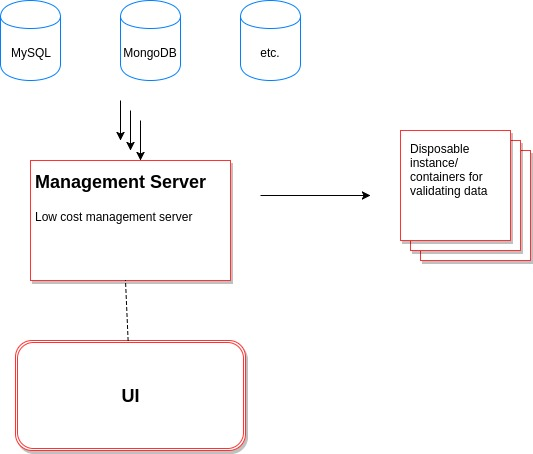
\includegraphics[scale=0.5,keepaspectratio]{diagram}
			\label{fig:diagram}
		\end{figure}
		
		\noindent \textbf{Management Server:} This will be a small low cost AWS instance on which the Jenkins automation server will be installed. The majority of the systems functionality will be carried out and/or orchestrated by this server. Jenkins jobs will copy the backups from their location to a disposable instance and implement the necessary steps to validate them such as importing and and reading.
		
		\noindent \textbf{User Interface:} This will provide a simple user interface (UI) for the system, implemented as a simple web app, hosted on AWS.It will allow users with little knowledge of Jenkins and AWS to perform backup restoration checks by adding a layer of abstraction. Users will be able to run restorations by providing the parameters such as the backup file and it's location. The UI will utilise the Jenkins API to run execute the restoration with the parameters provided.
		
		\noindent\textbf{Disposable Instances or Containers:} Disposable infrastructure will be used to perform the restoration. EC2 instances or containers can be used to quickly and easily deploy the necessary software to perform the restoration (i.e. the correct DB management system). They can also be destroyed afterwards, destroying the data and therefore maintaining confidentiality.

	\subsection{Formal Modelling}
	\subsubsection{Sequence Diagrams}
	
		The main function of the systems have been demonstrated below in sequence diagrams. \autoref{fig:seq-run-restore} shows the process of running a single backup restore. This involves a user manually triggering a restoration using the web interface. The trigger a Jenkins job automates the remaining steps. The backup is copied from the backup server to the test restoration server where it is imported to a Database Management System such as MongoDB. A read of the data is then performed to verify that the data is uncorrupted and readable. Finally it is detroyed from the restoration server.
		\begin{figure}[H]
			\setlength{\belowcaptionskip}{15pt plus 3pt minus 2pt}
			\caption{Run Restore}
			\centering
			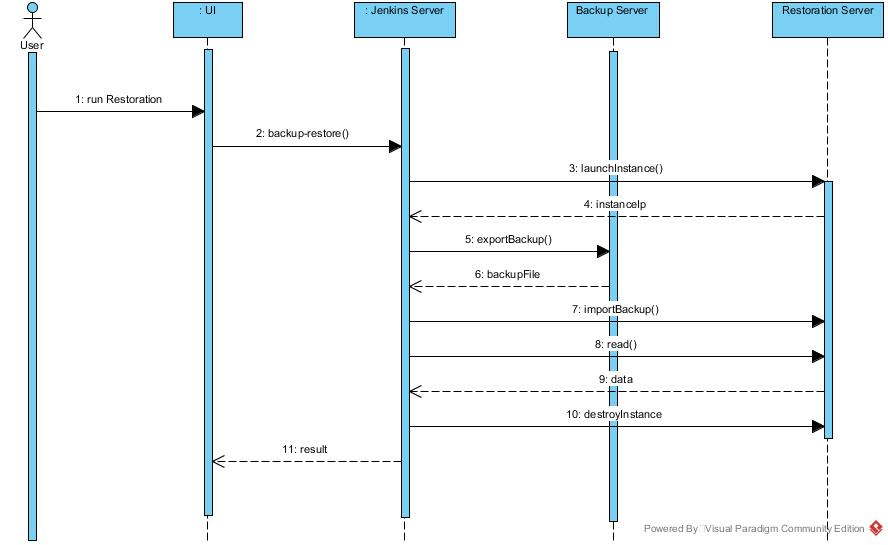
\includegraphics[width=\textwidth,keepaspectratio]{sequence-diagram-run-restore}
			\label{fig:seq-run-restore}
		\end{figure}

		\noindent \autoref{fig:seq-schedule-restore} shows the process of a scheduling regular backup restoration tests. Again, this is triggered by a user from the web interface. The web interface will passes the JSON or xml configuration for a job to the Jenkins server. The server will then create and save the job. A status indicating whether the job was created successfully is returned to the user. 
		\begin{figure}[H]
			\setlength{\belowcaptionskip}{15pt plus 3pt minus 2pt}
			\caption{Schedule Regular Restore}
			\centering
			%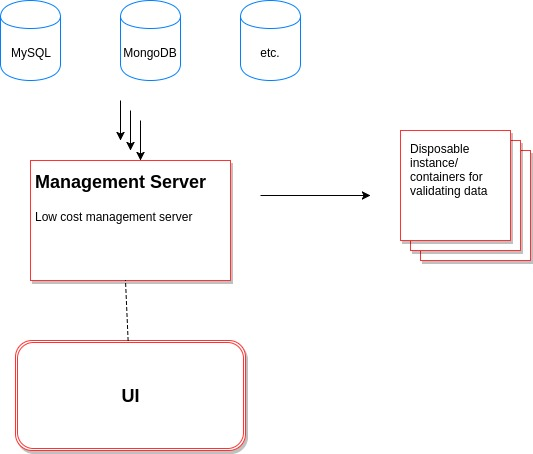
\includegraphics[width=\textwidth,height=\textheight,keepaspectratio]{diagram}
			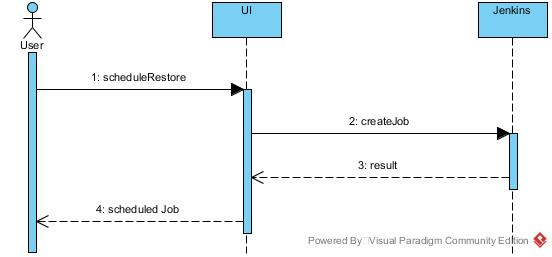
\includegraphics[width=\textwidth,keepaspectratio]{sequence-diagram-schedule-restore}
			\label{fig:seq-schedule-restore}
		\end{figure}
		
		\noindent \autoref{fig:seq-delete-restore} Show the process of deleting an existing scheduled job. This is required if a user not longer want to run scheduled restoration of a particular backup (for example if that backup is non longer needed and deleted). The user must delete the job on the Jenkins server in order to prevent further attempted restorations running. The user triggers this process from the web interface. This sends a delete commands to the Jenkins server via the API to remove the schedule job. The status of the command, indicating a successful or failed restore, is returned to the user. 
		\begin{figure}[H]
			\setlength{\belowcaptionskip}{15pt plus 3pt minus 2pt}
			\caption{Delete Scheduled Restore}
			\centering
			%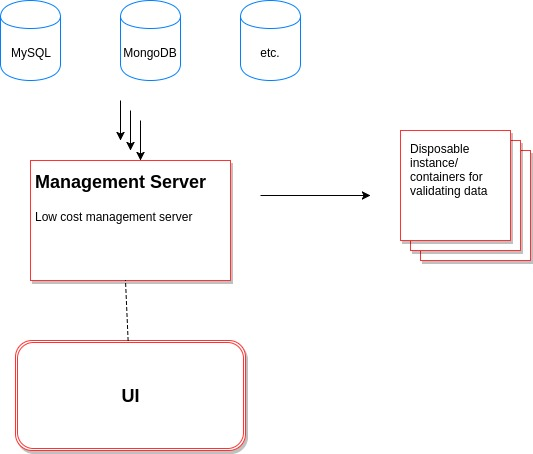
\includegraphics[width=\textwidth,height=\textheight,keepaspectratio]{diagram}
			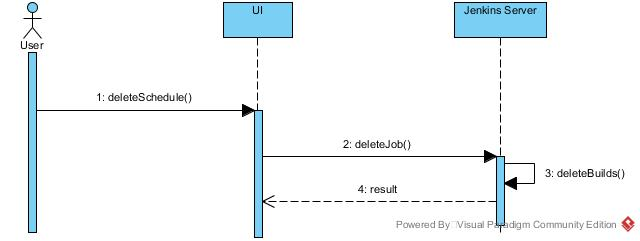
\includegraphics[width=\textwidth,keepaspectratio]{sequence-diagram-delete-schedule}
			\label{fig:seq-delete-restore}
		\end{figure}
	
	\subsubsection{User Stories}
		User stories are provided in \autoref{table:user-stories}. These the stories for general user such as running and scheduling restores. Also included are administration user stories. As system is create and destroys infrastructure on AWS, it would be necessary to limit access to the system.
		
		\begin{table}[H]
			\setlength{\belowcaptionskip}{15pt plus 3pt minus 2pt}
			\caption{User Stories}
			\begin{tabular}{|l|p{0.4\linewidth}|p{0.4\linewidth}|} \hline
				\textbf{As a} & \textbf{I want to} & \textbf{so that} \\ \hline
				manager & be able to add/remove my team members to the system & they can test backups \\ \hline
				user & perform a restoration of a database backup & I can verify the backup restore process works \\ \hline
				user & view the results of a backup restore & I can verify the backup contains valid, readable data \\ \hline
				user & schedule a regular automated restoration of a particular backup & I don't have to manually do it myself \\ \hline
				user & view the results of an automated restoration check & I can verify the backup contains valid, readable data \\ \hline
				user & view past results of all automated checks & I can keep track of successful and unsuccessful restorations \\ \hline
				user & be easily notified when a restoration fails & promptly address the issue a possible backup failures \\  \hline
			\end{tabular}
			\label{table:user-stories}
		\end{table}
		
	\subsection{Front End Design}
	\subsubsection{Wireframes}
		\begin{figure}[H]
			\setlength{\belowcaptionskip}{15pt plus 3pt minus 2pt}
			\caption{Homepage}
			\centering
			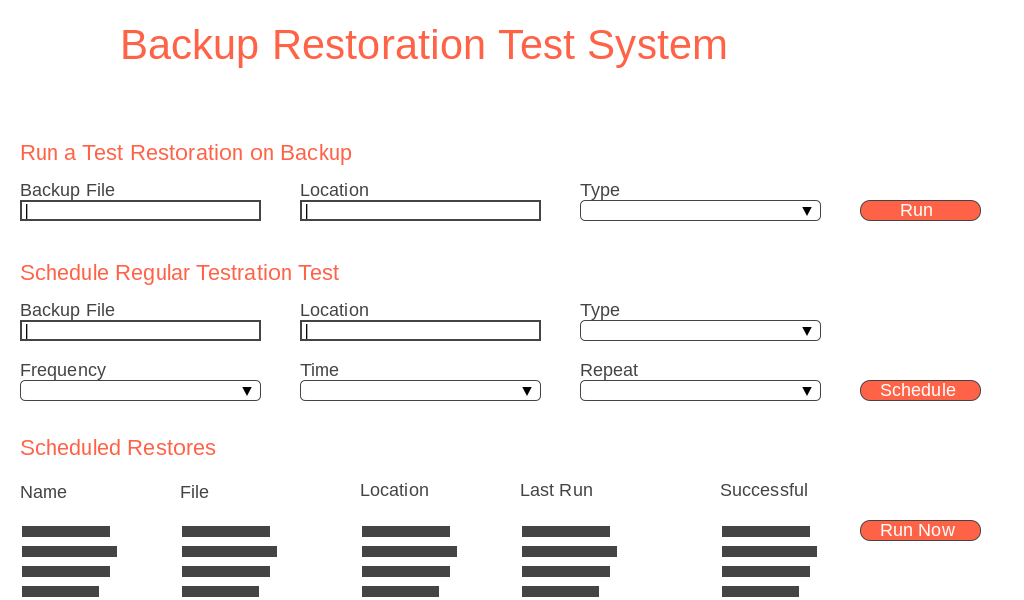
\includegraphics[width=\textwidth,keepaspectratio]{wireframe-homepage}
			\label{fig:homepage}
		\end{figure}
		
		\begin{figure}[H]
			\setlength{\belowcaptionskip}{15pt plus 3pt minus 2pt}
			\caption{Scheduled Restore}
			\centering
			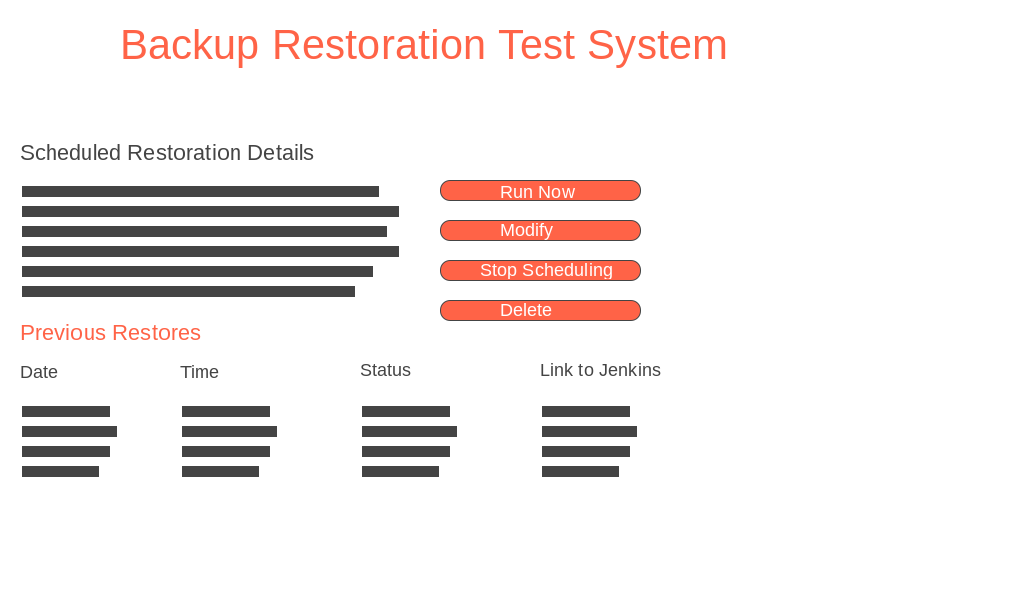
\includegraphics[width=\textwidth,keepaspectratio]{wireframe-scheduled-restore}
			\label{fig:scheduled}
		\end{figure}
	
	